\subsection{Evaluation the forecasting performance}
In that section, we first evaluate the quality of the forecasting step. That one depends on at least two parameters:
\begin{itemize}
\item The noise variance $\sigma^2$.
\item The size of the training dataset $K$. 
\end{itemize}
In subsections~\ref{ssse:res.sine} and~\ref{ssse:res.ahm}, we study the influence of these parameters. A comparison with the theoretical results of section~\ref{se:theoretical} is also available.

\subsubsection{Sum of sine waves}
\label{ssse:res.sine}
We proved that the linear dynamic model is sufficient to catch the dynamical behavior of signals taking the form~\eqref{eq:sum.sine}. In order to validate this theoretical result, we apply the forecasting Algorithm~\ref{alg:extension} to a large number of realizations of the random vector $\bz$ such that:
\[
\bz = \bx+ \sigma\bw\ ,
\]
where
\[
\bx[n] =\cos\left(2\pi p_1 \dfrac{n}{M} \right) + R\cos\left(2\pi p_2 \dfrac{n}{M} \right)\ ,\quad\forall\ n\in\{1,\ldots,N\}\ ,
\]
and $N=10^4$, $M=750$, $p_1=10$, $p_2=33$ and $R=1.4$. Besides, the additive noise is chosen to be Gaussian: $\bw\sim\cN(\bzero,\bI)$.

\paragraph{Influence of the noise variance $\sigma^2$.} Here, the size of the training dataset is set to $K=1875$. Then, the forecasting algorithm is run on 100 realizations on the discrete signal $\bx$ for 100 different values of $\sigma^2$  logarithmically spaced from $5.10^{-3}$ to $10^{-1}$. For each of these values, we determine the experimental bias $\mu_{xp}[\ell]$ and variance $\gamma_{xp}[\ell,\ell]$ in function of the forecasting sample index $\ell$ (going from 1 to $L=500$). These results are displayed on Figure~\ref{fig:res.noise.sine}. Each color corresponds to these experimental results obtained for a given value of $\sigma$. On the left of Figure~\ref{fig:res.noise.sine}, the result show that the bias is neither depending on the noise variance $\sigma^2$ nor the forecasting length $\ell$, and always insignificant with respect to the signal values. On the right of Figure~\ref{fig:res.noise.sine}, we display the normalized experimental variance, that is $\frac{\gamma[\ell,\ell]}{\sigma^2}$. This highligths the fact that the forecasting variance increases linearly with respect to $\sigma^2$. More surprisingly, this result shows that the forecasting variance decreases with $\ell$, what is counterintuitive.  
\begin{figure}
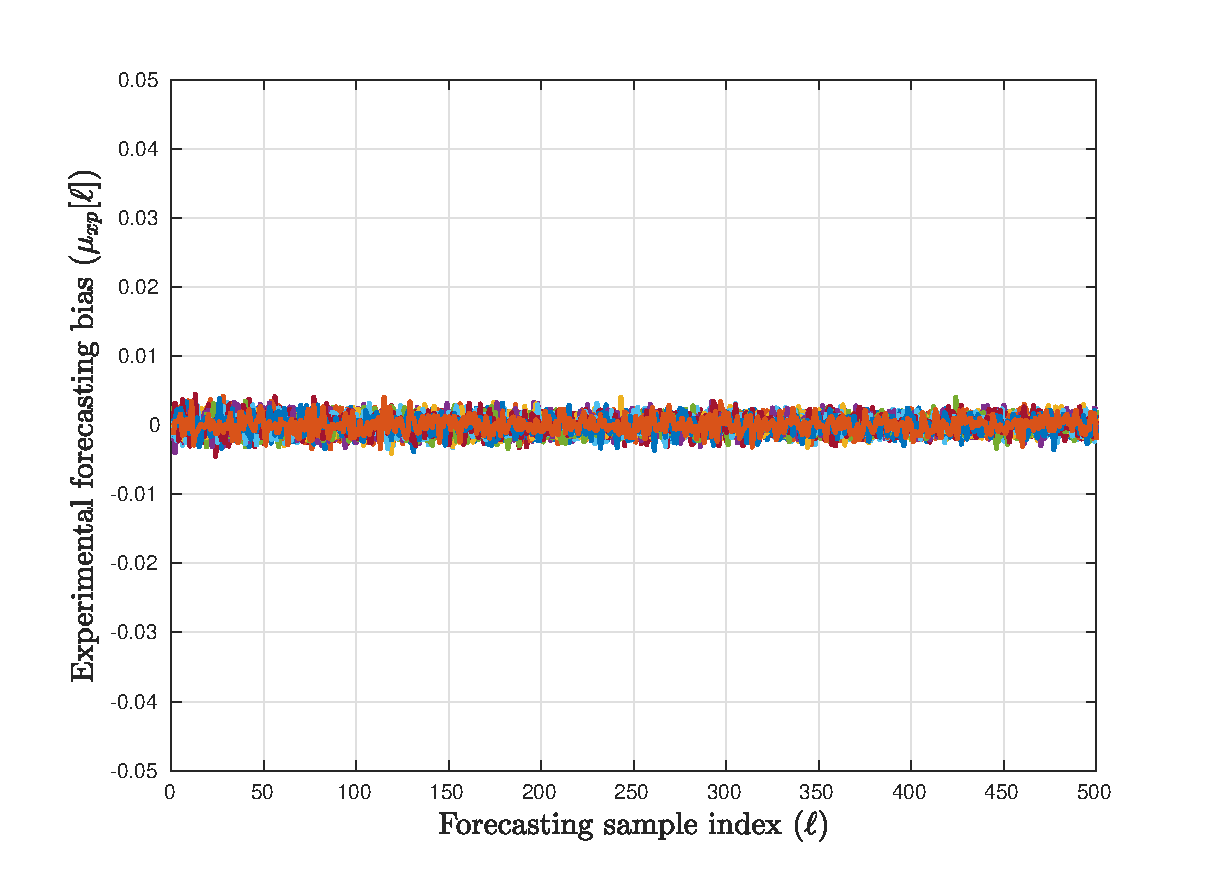
\includegraphics[width=.49\textwidth]{biasNoiseSine.eps}
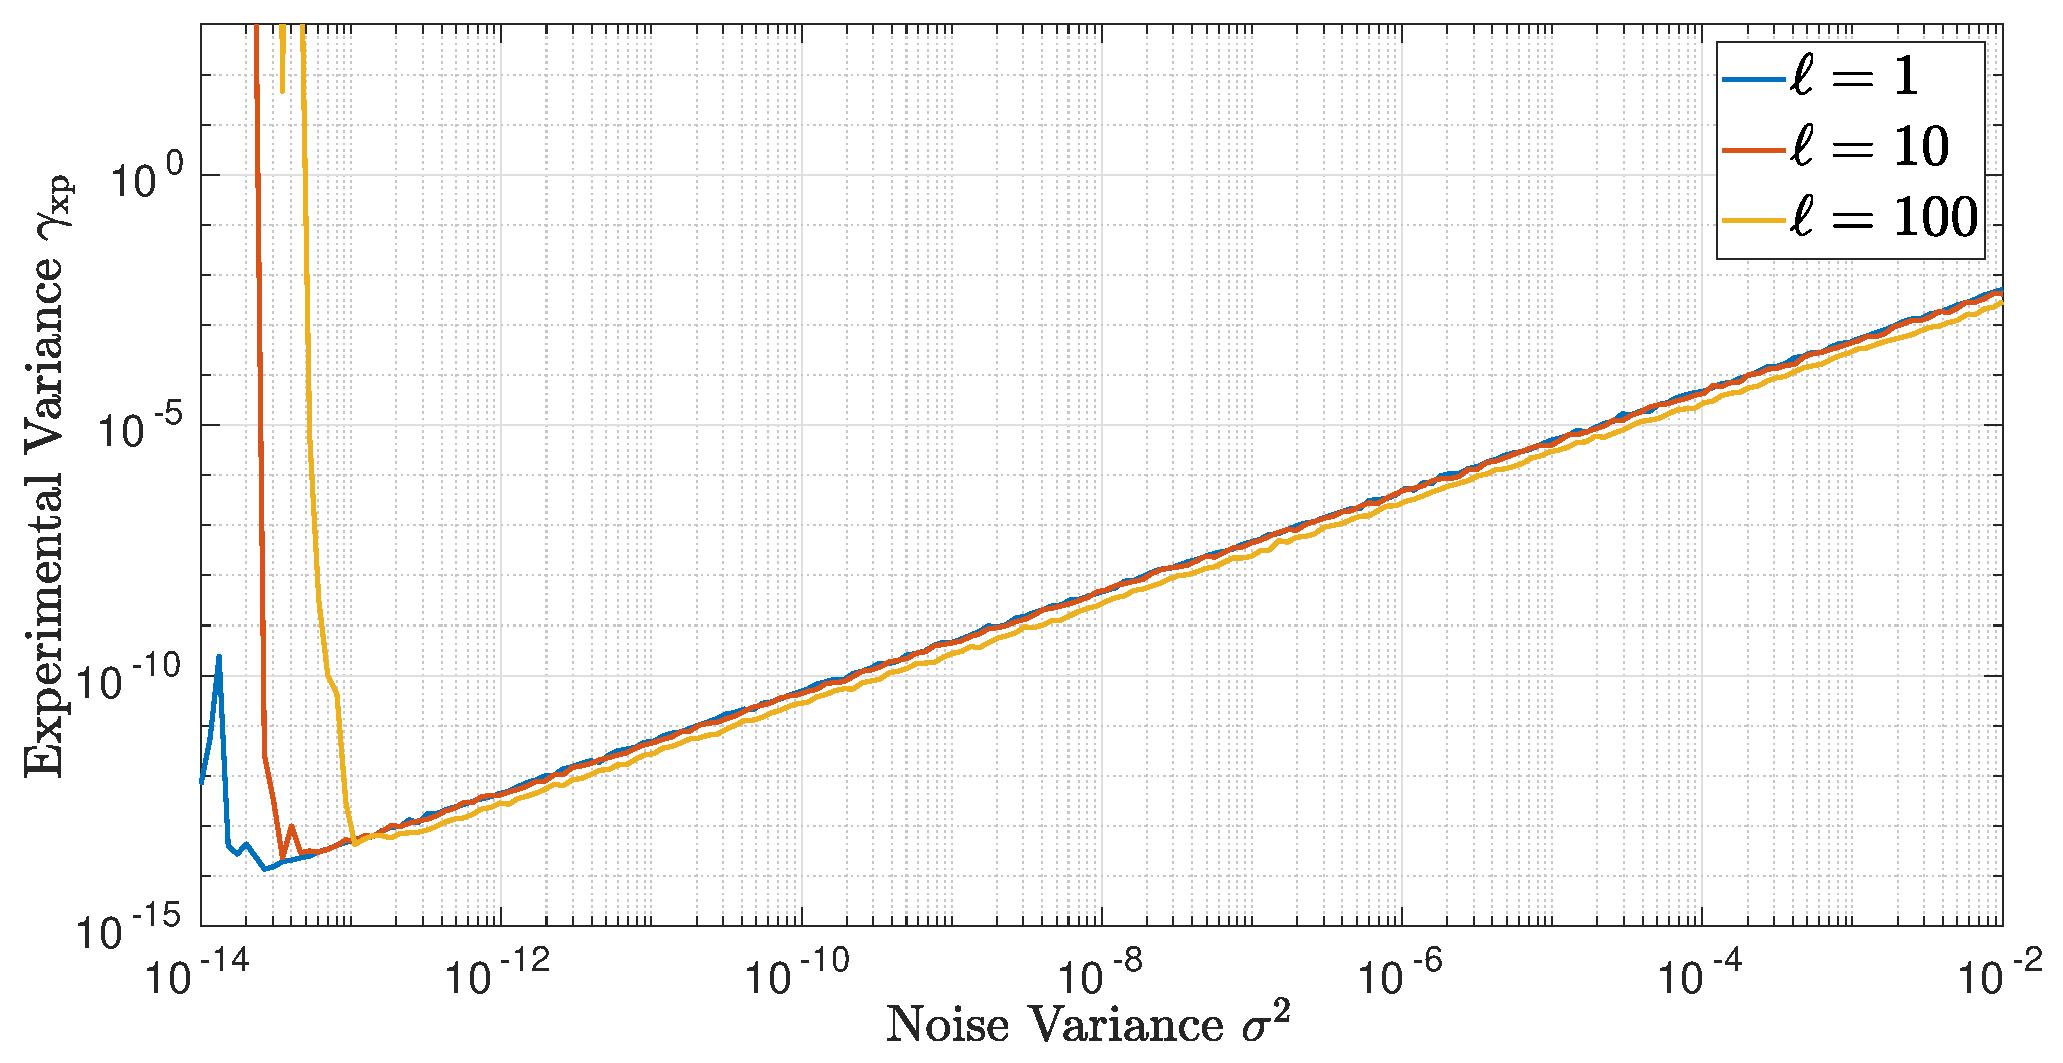
\includegraphics[width=.49\textwidth]{VarianceNoiseSine.eps}
\caption{Evolution of the experimental forecasting bias (left) and the normalized forecasting variance (right) in function of the forecasting sample index. Each color characterizes the result for a given value of $\sigma$.}
\label{fig:res.noise.sine}
\end{figure}

\paragraph{Influence of the training dataset size $K$.} Here, the noise variance $\sigma$ is set to $\sigma=10^{-2}$. Then, the forecasting algorithm is run on 3000 realizations on the discrete signal $\bx$ for 25 different values of $K$, logarithmically spaced from $3.5\times 10^{3}$ to $6\times 10^{3}$. For each of these values, we determine the experimental bias $\mu_{xp}[\ell]$ and variance $\gamma_{xp}[\ell,\ell]$ in function of the forecasting sample index $\ell$ (going from $1$ to $500$). These results are displayed on Figure~\ref{fig:res.size.sine}. Each color corresponds to these experimental results obtained for a given value of $K$. On the left of Figure~\ref{fig:res.size.sine}, as expected, the experimental bias vanishes. On the right of Figure~\ref{fig:res.size.sine}, we display the product of $K$ with the normalized experimental variance, that is $\frac{\gamma[\ell,\ell]}{\sigma^2}$. This result shows the asymptotic behavior of the variance. Indeed, as soon as $K$ is sufficiently high, the product $K\gamma[\ell,\ell]$ is approximately independent of $K$.
\begin{figure}
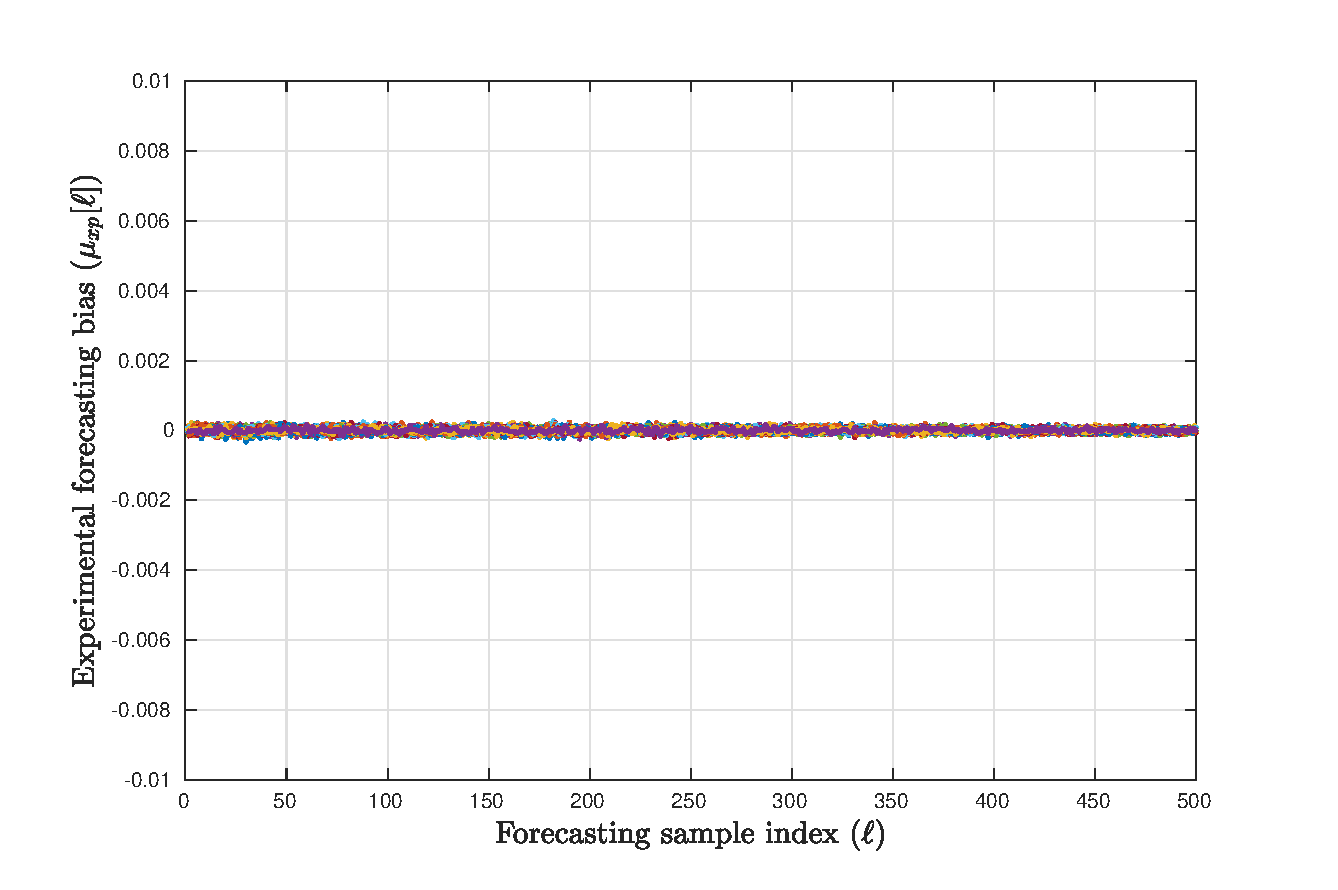
\includegraphics[width=.49\textwidth]{BiasKSine.eps}
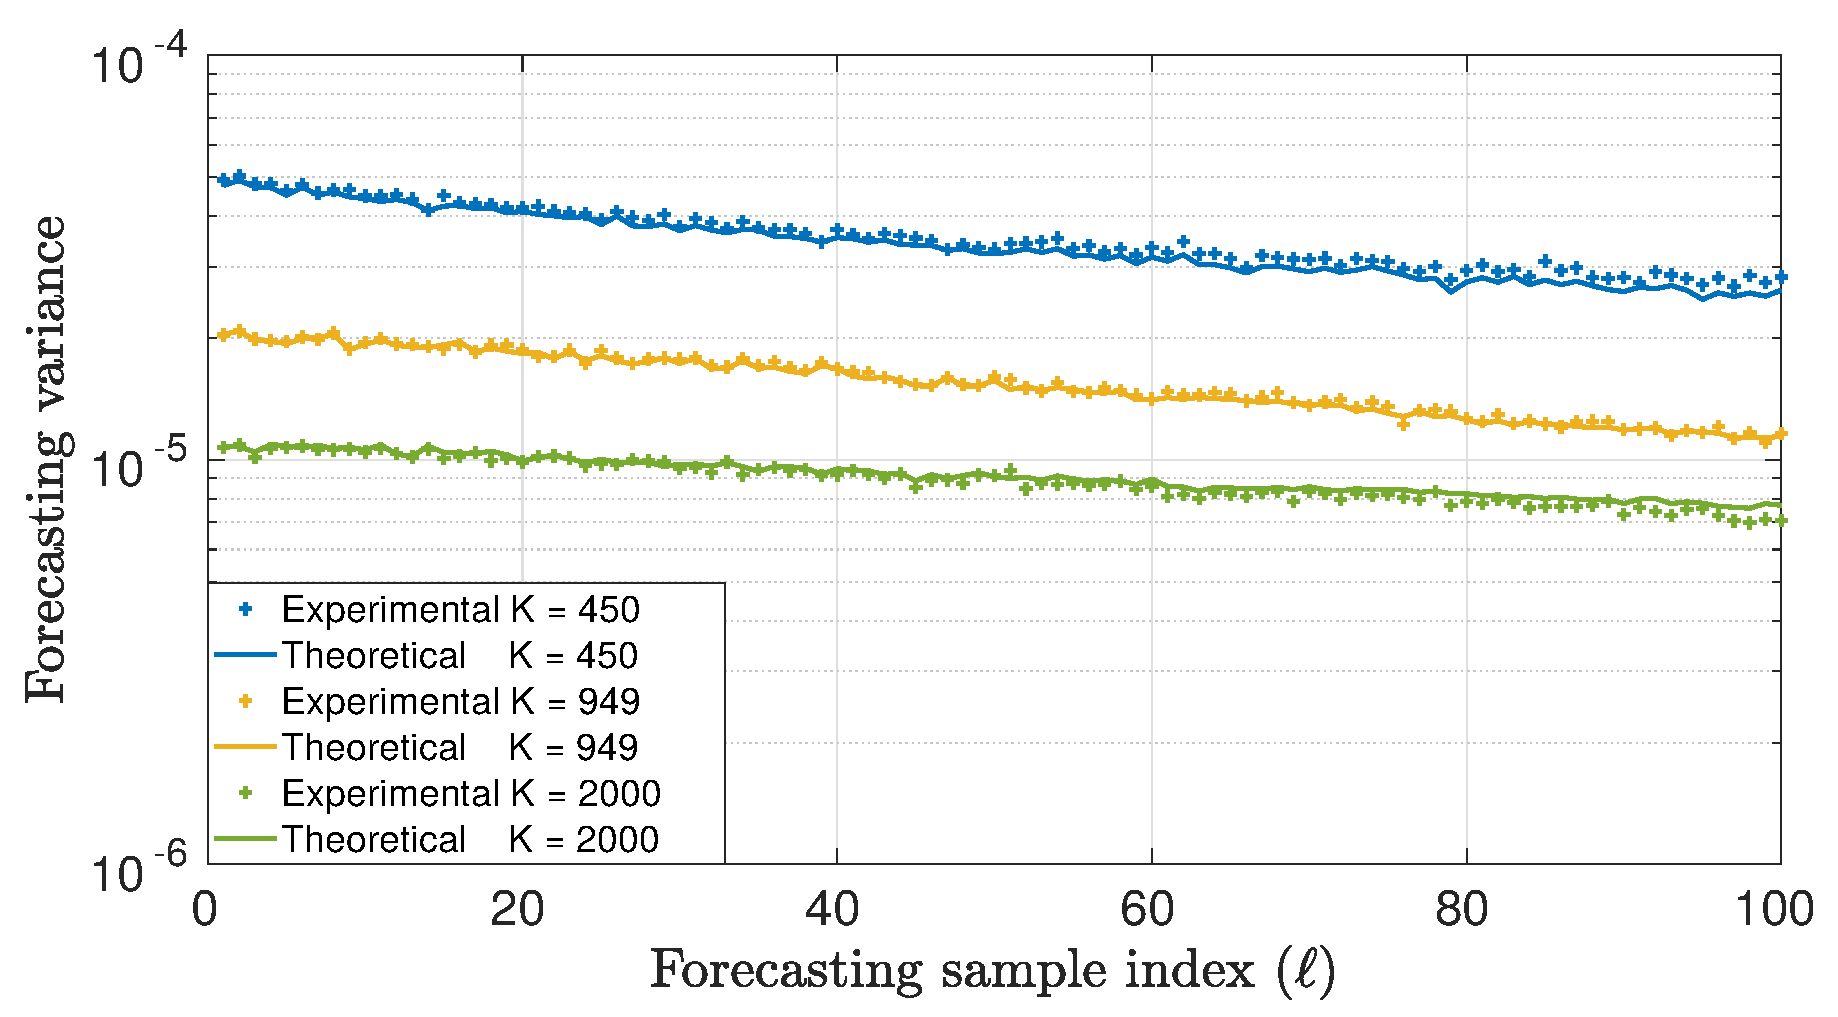
\includegraphics[width=.49\textwidth]{VarianceKSine.eps}
\caption{Evolution of the experimental forecasting bias (left) and the normalized forecasting variance (right) in function of the forecasting sample index. Each color characterizes the result for a given value of $K$.}
\label{fig:res.size.sine}
\end{figure}

\paragraph{Conclusion.}
Both previous results allows us to describe the influence of the noise variance and the size of the training dataset on the variance of the forecasting noise, which is empirically summarized as follows:
\begin{equation}
\gamma[\ell,\ell] \sim \dfrac{\sigma^2}{K}g[\ell] \ ,\quad\mbox{when}\ \sigma^2\to 0\ \mbox{and}\ K\to\infty \ ,
\end{equation} 
where $g$ is a bounded positive function.

\subsubsection{Adaptive harmonic model}
\label{ssse:res.ahm}
We now consider a signal whose instantaneous frequencies and amplitudes of its components vary over time. The toy signal we use takes the following form:
\[
\bx[n] = \cos\left(2\pi \phi_1[n] \right) + R[n]\cos\left(2\pi \phi_2[n] \right)\ ,\quad\forall\ n\in\{1,\ldots,N\} \ ,
\] 
where the instantaneous amplitude $R$ is given by:
\[
R[n] = 1.4 + 0.2\cos\left(4\pi\frac{n}{N}\right)\ ,
\]
and the instantaneous phases are such that:
\begin{align*}
\phi_1[n] &= \frac{p_1}{M}\left( n + \frac{0.01}{2\pi}\cos\left(2\pi\frac{n}{N}\right) \right) \\
\phi_2[n] & = p_2\frac{n}{M} + \frac{20}{2N\fs}n^2
\end{align*}
Besides, the additive noise is chosen to be Gaussian: $\bw\sim\cN(\bzero,\bI)$. Numerically, we take: $N=10^4$, $M=750$, $p_1=10$, $p_2=23$ and $R=1.4$.

To highlight the fact that the linear dynamical model is sufficient to catch most of the dynamical behavior of signals following the AHM, we compare the performance of the Algorithm~\ref{alg:boundary} with reference forecasting algorithm that could be used for extending such signals. These methods are:
\begin{itemize}
\item The \emph{Extended Dynamic Mode Decomposition (EDMD)} has been developped by Williams \etal~\cite{Williams15data}. The proposed algorithm is a way to obtain an approximation of the so-called Koopman operator of the observed system, which theoretically allows to catch dynamic of nonlinear systems~\cite{Korda18linear}.
\item The \emph{Gaussian Process Regression (GPR)}~\cite{Rasmussen06gaussian} is a method relying on a probabilistic dynamical model. That one is based on the Gaussian process structure, and therefore offer more flexibility in the type of dynamic that could be modeled than the linear model~\eqref{eq:dyn.model}. 
\end{itemize}

To quantify the global quality (\ie~not depending on $\ell$) of the forecasting approaches, we evaluate the Experimental Mean Square Error $\mathrm{MSE_{xp}}(\tilde\bx)$ of the forward forecast extended signals, namely:
\begin{align}
\label{eq:mse}
\mathrm{MSE_{\xp}}(\tilde\bx) &= \dfrac1{L}\|\tilde\bx -\bx^\mathrm{ext}\|^2 \\
\nonumber
&= \dfrac1{L}\sum_{\ell=1}^L \bmu_{\xp}[\ell]^2 + \bgamma_{\xp}[\ell,\ell]\ .
\end{align}
where $\bx^\mathrm{ext}$ is the ground-truth extended signal, that is: $\bx^\mathrm{ext} = \begin{pmatrix}\bx[-L] & \cdots & \bx[N-1+L] \end{pmatrix}$. Then, as long as the bias $\bmu[\ell]$ and the variance $\bgamma[\ell,\ell]$ of the forecasting estimator remain small for all $\ell$, the MSE takes small values either. Corresponding results are given in Table~\ref{tab:mse.sine}. They show that the naive extension we propose gives satisfying results, even though the oher methods, more sophisticated gives MSE values that are somewhat smaller. Netherveless, a major limit of those methods is the computing time they require, which prevent them from being used to exploit real-time data. Thus, {\sf SigExt} is the method that optimize the trade-off between the forecasting quality and the computing time as extension method. That is why, it is implemented in our algorithm for the reduction of boundary effect.

\begin{table}
\centering
\caption{Performance of the extension methods.}
\begin{tabular}{|c||c|c|c|}
  \hline
   \multirow{2}{*}{Algorithm} & \multicolumn{2}{c|}{MSE}  & \multirow{2}{*}{Computing time (sec.)} \\
   \cline{2-3} & Mean & Standard deviation & \\
   \hhline{|=#=|=|=|}
   {\sf SigExt} & $1.433\times 10^{-3}$ & $4.361\times 10^{-4}$ & $0.15$ \\
   \hline
   EDMD & $3.076\times 10^{-2}$ & $8.095\times 10^{-2}$ & $2.53$\\
   \hline
   GPR & $1.436\times 10^{-3}$ & $4.346\times 10^{-4}$ & $146.33$ \\
   \hline
\end{tabular}
\label{tab:mse.sine}
\end{table} 


\subsection{Evaluation of the quality of the boundary effect reduction}

\subsubsection{Metrics}
The quality of the boundary effect reduction must be evaluated on the synchrosqueezing representation. To that aim, we compare the obtained synchrosqueezing transform to the optimal synchrosqueezing transform $\ccF_N^\mathrm{opt}(\bx)$. The optimal synchrosqueezing transform is defined as the restriction of the synchrosqueezing of the ground-truth extended signal $\bx^\mathrm{ext}$. Therefore, we have:
\begin{equation*}
\ccF_N^\mathrm{opt}(\bx) = \cR\left( \ccF_{N+2L}(\bx^\mathrm{ext}) \right) \ .
\end{equation*} 

The different representations we obtained must be compared to the optimal SST. To that aim, we establish a criterion that quantify the distance of these time-frequency representations to the optimal one. To do this, we reason in analogy with the optimal transport distance which allows us to quantify the distance between two probability density functions. Let us generically denote a time frequency representation $\ccQ$. Then, for $t$ fixed, we consider the following pseudo probability density function:
\begin{align}
p_\ccQ^t(\xi) &= \dfrac{|\ccQ(\xi,t)|^2}{\int_\RR |\ccQ(\nu,t)|^2\dd\nu}\ .
\label{eq:ppdf}
\end{align}
Similarly, let $p_{\ccF_0}^t$ denotes the associated pseudo-probability density function (defined as in~\eqref{eq:ppdf}) associated with the reference time-frequency representation $\ccF_0$. At each instant $t$, we can then determine the optimal transport distance $d_{t}$ between the two pseudo densities. It is given by the $L^1$ norm of the difference between the associated distribution functions. In other words, either $P_{\ccQ}^t(\xi)=\int_{-\infty}^\xi p_{\ccQ}^t(\nu)\dd\nu$ and $\tilde P_{\ccF_0}^t(\xi)=\int_{-\infty}^\xi\tilde p_{\ccF_0}^t(\nu)\dd\nu$, we have
\begin{equation*}
d_{t}(\ccQ,\ccF_0) = \int_\RR\left|\tilde P_{\ccQ}^t(\xi)-  P_{\ccF_0}^t(\xi)\right|\dd\xi\ .
\end{equation*}
Finally, the distance between the two time-frequency representations is obtained by averaging all the optimal transport distances with respect to time:
\begin{equation}
D(\ccQ,\ccF_0) = 100\times\frac1{|I|}\int_I d_{t}(\ccQ,\ccF_0)\dd t\ .
\end{equation}
The \textit{Optimal Transport Distance} (OTD) quantifies the proximity between the estimated and actual instantaneous frequencies while favouring the sparsity of the estimated time-frequency representation.

\subsubsection{Respiratory signal}

The signal is 50 minutes-long and is sampled at $\fs=100$~Hz. A zoom on a small portion of the signal is displayed in Figure~\ref{fig:tho}.

\begin{figure}
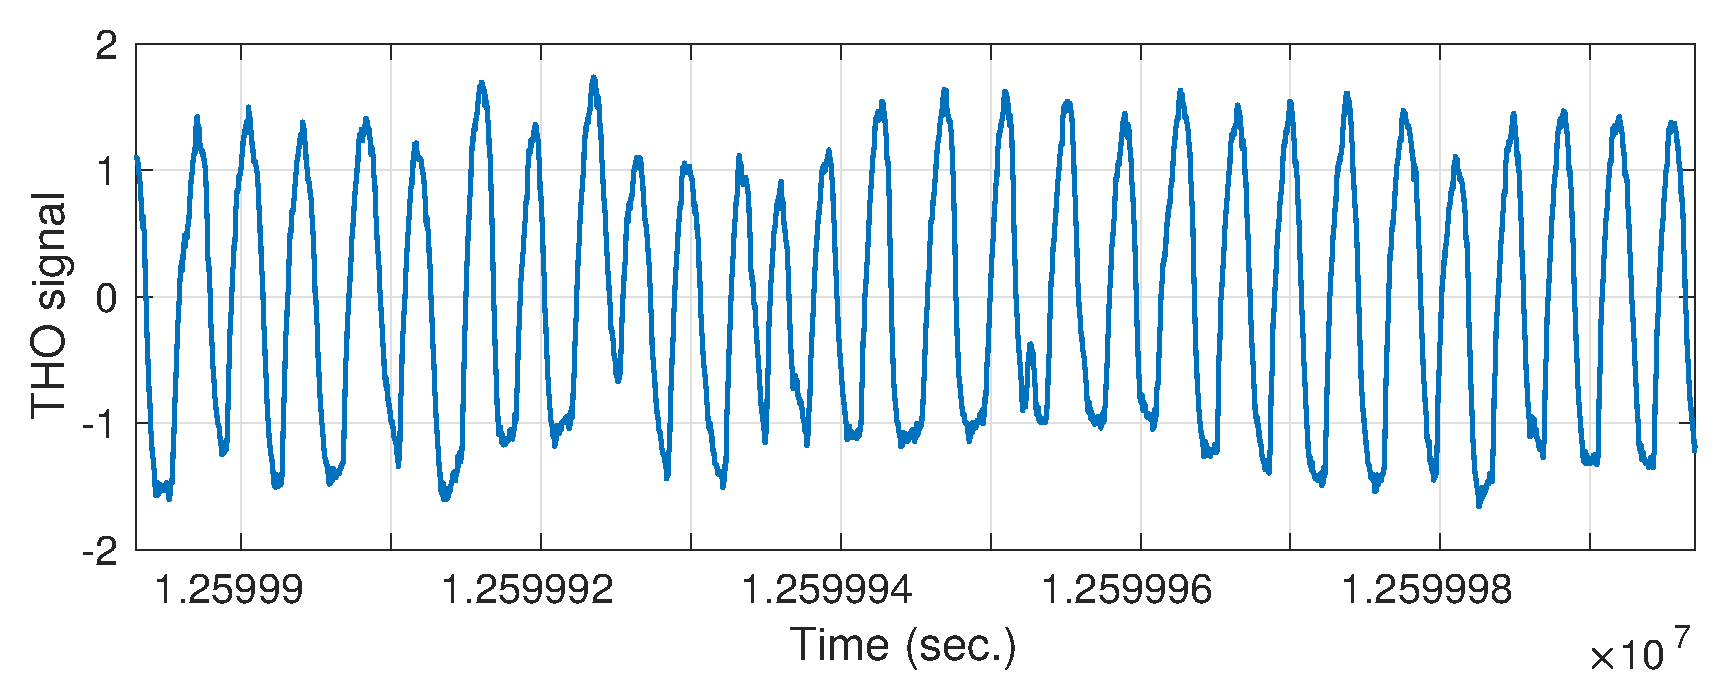
\includegraphics[width=\textwidth]{THOsig.eps}
\caption{Zoom on the respiratory signal.}
\label{fig:tho}
\end{figure}

From that large signal, we build a dataset of $48$ non-overlapping signals of 60 seconds, \ie~$N=6000$. On each of these pieces of signal, we implement the Algorithm~\ref{alg:boundary} on diverse time-frequency and time-scale representations. The corresponding results are given in Table~ 

The forecasting Algorithm~\ref{alg:extension} is applied to each of the signals in the dataset we built. These ones are extended of 7 second on each border, corresponding to $L =700$. Thus, in order to catch slowly varying dynamical behaviors, the size of the training signal $M$ is chosen so that $M=\lfloor 1.5L\rfloor$. As a result of section~\ref{ssse:res.sine}, we take: $K=\lfloor2.5M\rfloor$. The average and the standard deviation of the MSE~\ref{eq:mse} with respect to the simulations are given in Table~\ref{tab:mse}.

\begin{table}
\centering
\caption{Averaged MSE.}
\begin{tabular}{|c||c|c|}
  \hline
   \multirow{2}{*}{Algorithm} & \multicolumn{2}{c|}{MSE} \\
   \cline{2-3}
      & Mean & Standard deviation\\
   \hhline{|=#=|=|}
   {\sf SigExt} & $0.7935$ & $0.2615$ \\
   \hline
   Zero padding & $0.9903$ & $0.0579$ \\
   \hline
\end{tabular}
\label{tab:mse}
\end{table} 

The results are compared with the strategy consisting in a zero-padding extension of the signal. These results  show a significant improvement of the quality of the forecasting. Indeed, in average, the forecasting MSE is improved of almost $20\%$. Nevertheless, the variance forecasting MSE shows a huge variability in the quality of the estimation. This is probably due to the outliers and pulse that can be find in the respiratory signal. That ones make the adaptive harmonic model temporary irrelevant, and break the validity of the linear dynamic model.


Even though the performance of the forecasting algorithm is moderate, the boundary effect can be reduced dramatically on the time-frequency and time-scale representations. We evaluate the OTD to the optimal representation for different time-frequency and time-scale representation. Notice that the extension length $L$ is set accordingly to the window length used by the time-frequency analysis tool. For instance, here the window length we use to evaluate the STFT is of 1500 samples. To prevent the STFT from being sensitive to the boundary effect, we set $L=750$. In this way, when evaluating the spectral content of the signal near its boundaries, the analysis is not limited by a lack of information all along the window support. From now on, all results are given for $L$ at equal to the half of the width of the window used in the time-frequency transform.  

\begin{table}
\centering
\caption{Performance of the Boundary effect reduction on TFR.}
\begin{tabular}{|c||c|c|c|}
  \hline
   \multirow{2}{*}{Extension method} & \multicolumn{3}{c|}{Time-Frequency Representation} \\
   \cline{2-4}
      & STFT & SST & RS\\
   \hhline{|=#=|=|=|}
   Without extension & $2.16\times 10^{-2}$ & $5.26\times 10^{-3}$ & $3.07\times 10^{-2}$ \\
   \hline
   {\sf SigExt} & $1.72\times 10^{-2}$ & $4.00\times 10^{-3}$ & $2.43\times 10^{-2}$ \\
   \hline
   EDMD & $1.75\times 10^{-2}$ & $4.23\times 10^{-3}$ & $2.45\times 10^{-2}$ \\
   \hline
   GPR & $1.84\times 10^{-2}$ & $4.10\times 10^{-3}$ & $2.48\times 10^{-2}$ \\
   \hline
\end{tabular}
\label{tab:otd.tho}
\end{table}


\subsubsection{Photoplethysmogram}
\label{ssse:ppg}
We perform a study similar to the previous one on a 640 second-long photoplethysmogram (PPG) signal, sampled at $\fs=125$~Hz. A 32 second-long piece of this signal is displayed on the top of Figure~\ref{fig:ppg}. The estimated 2-second extension on both sides of this signal is superimposed to the ground-truth signal is provided on the bottom of Figure~\ref{fig:ppg}.

\begin{figure}
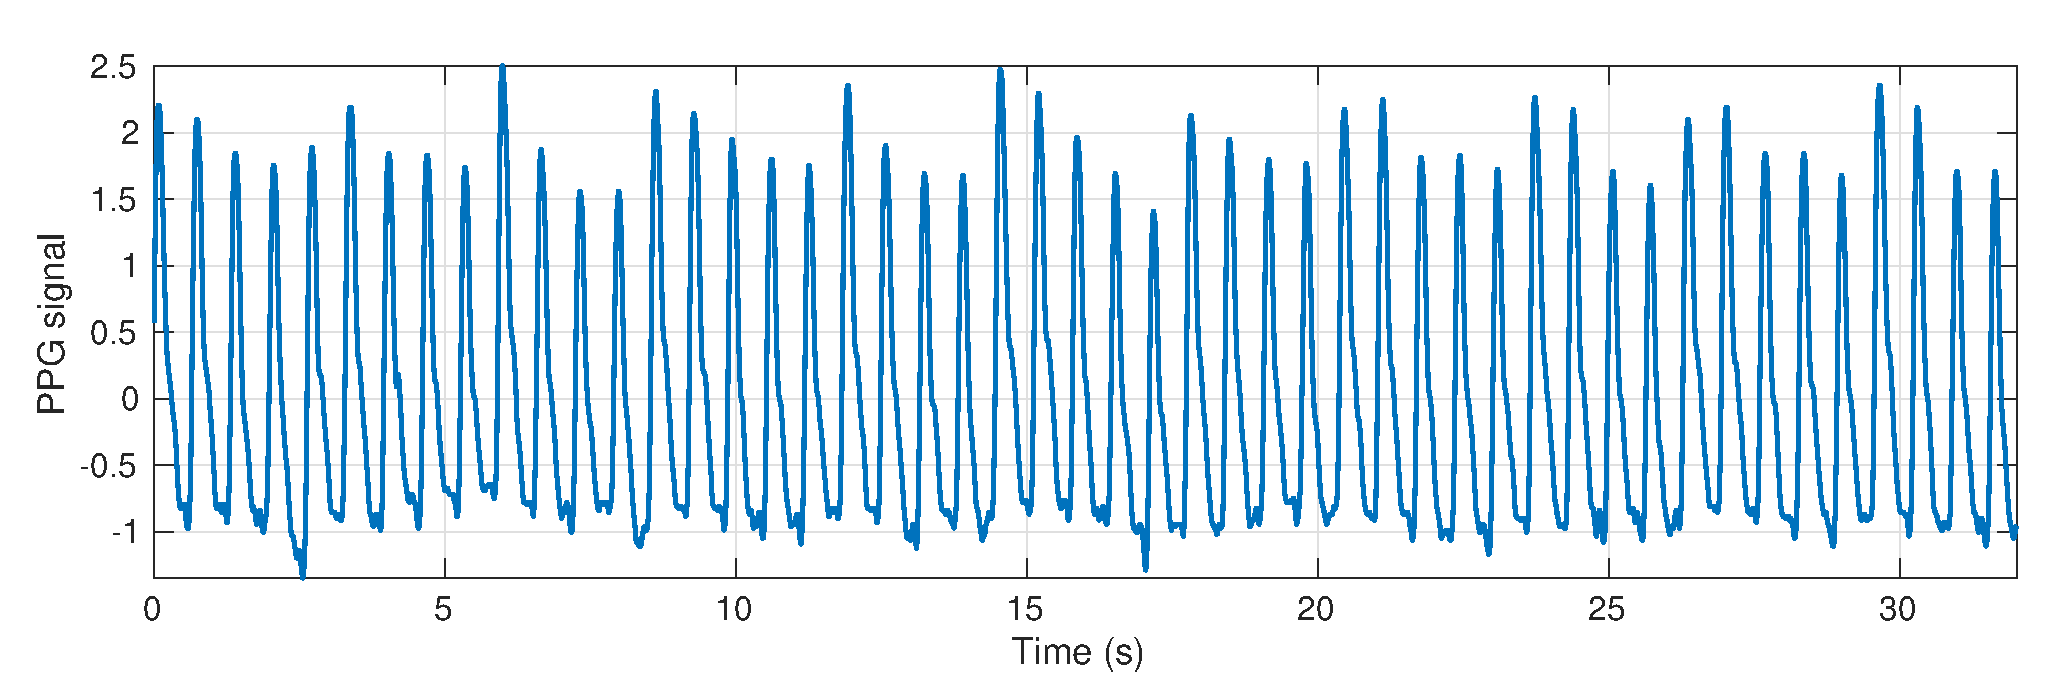
\includegraphics[width=\textwidth]{PPGsig.eps}
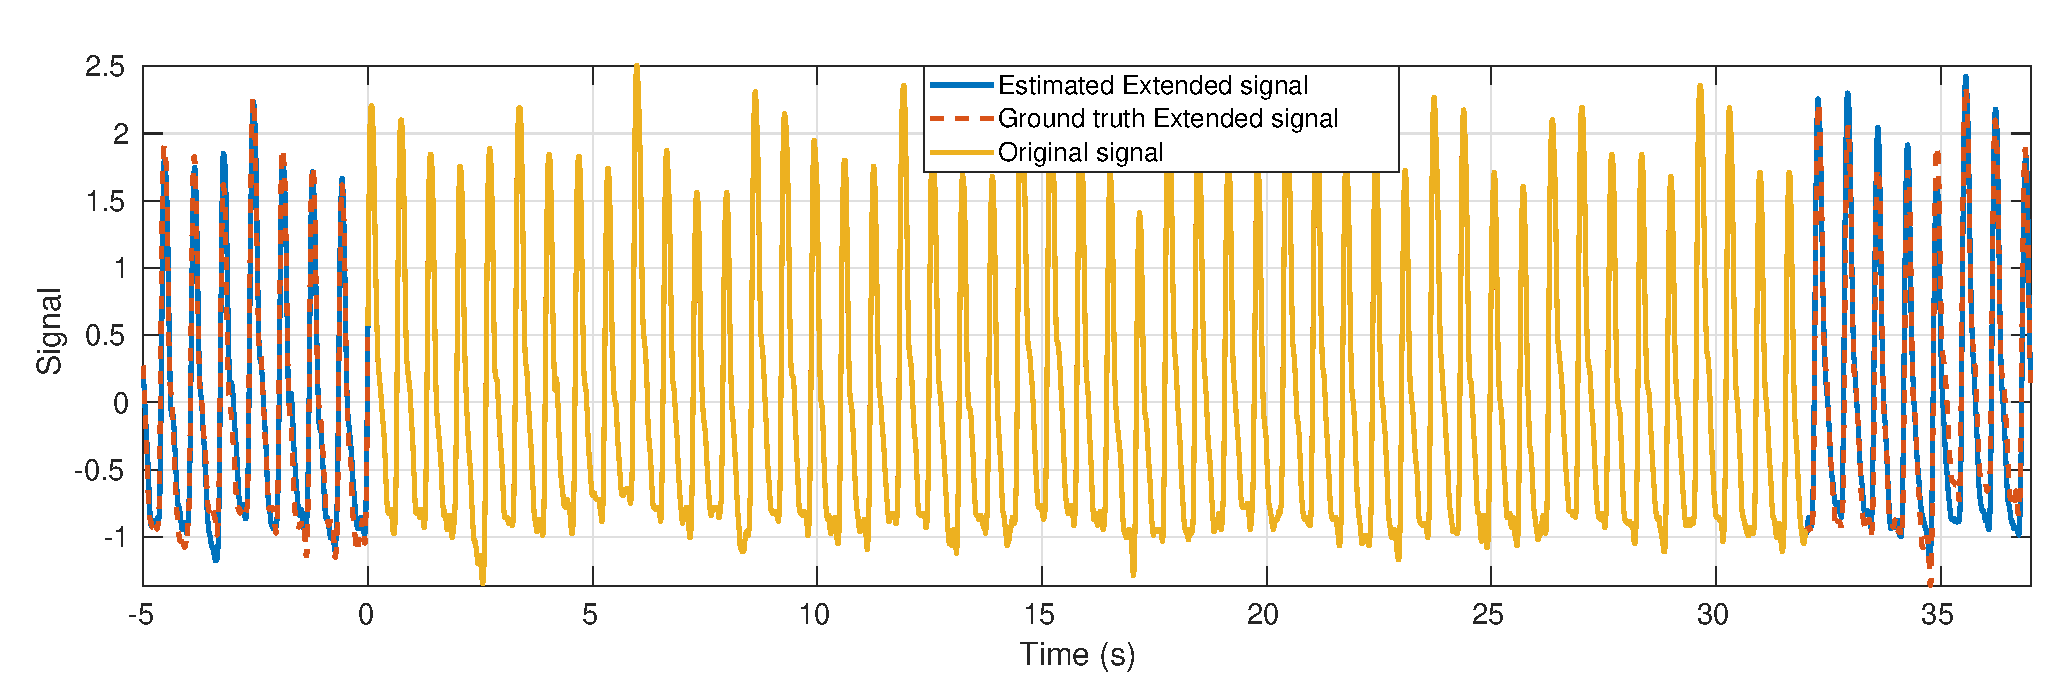
\includegraphics[width=\textwidth]{PPGforecast.eps}
\caption{PPG signal. Top: original measured signal. Extended signal obtained by forecasting superimposed with the ground truth signal.}
\label{fig:ppg}
\end{figure}

\begin{figure}
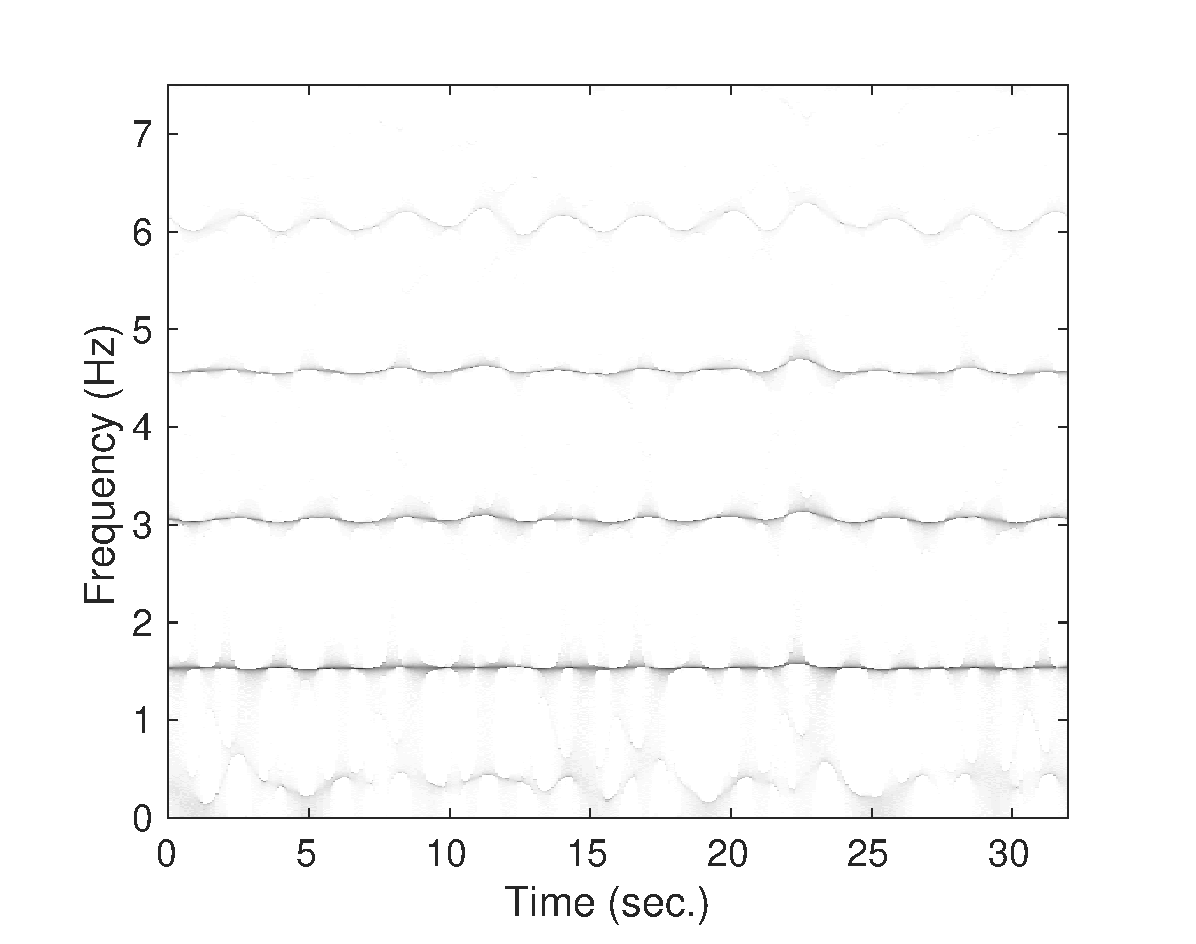
\includegraphics[width=.49\textwidth]{SSTBoundEffRed.eps}
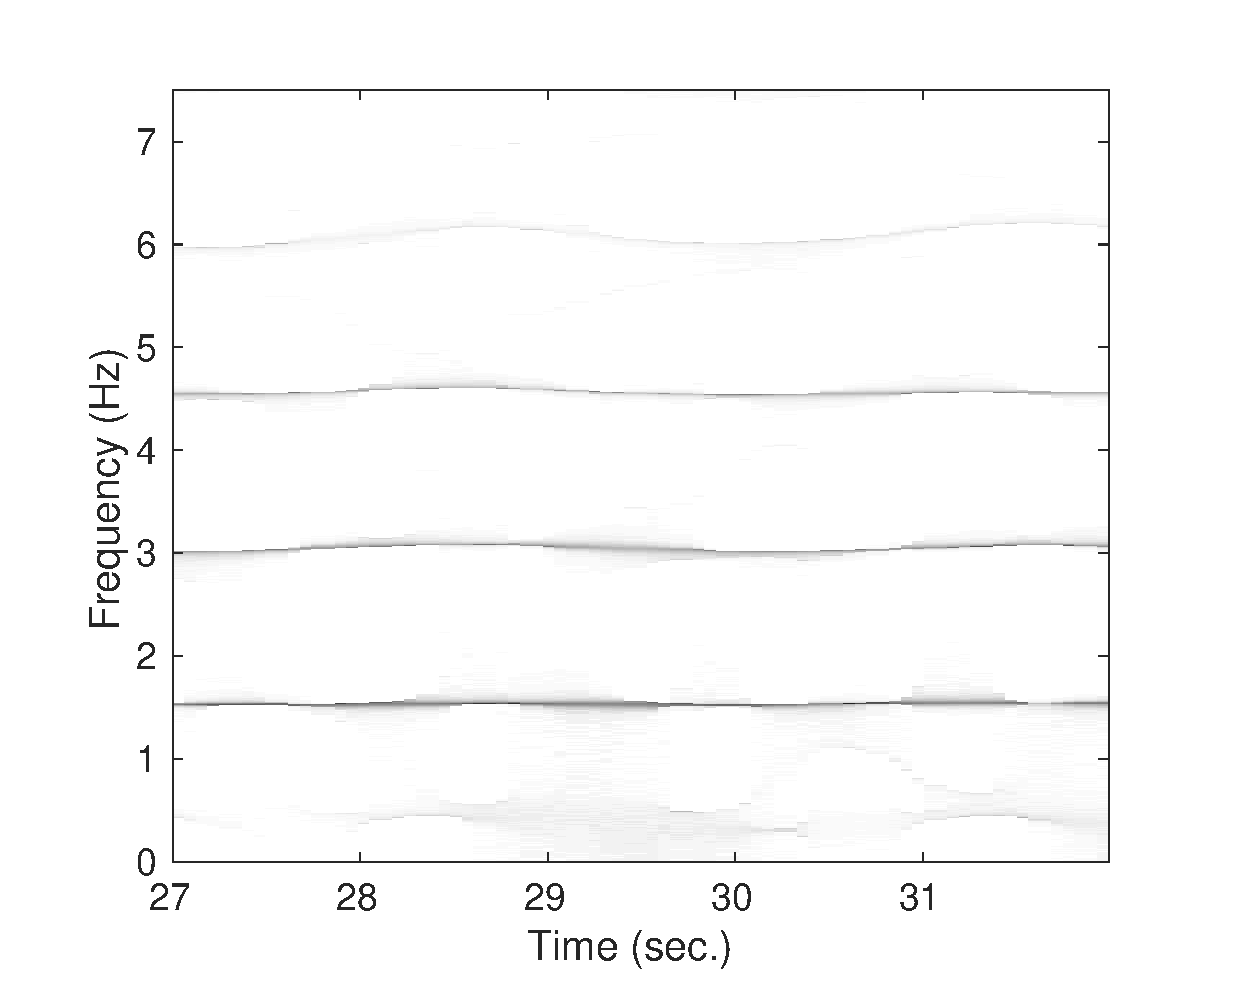
\includegraphics[width=.49\textwidth]{zoomSSTBoundEffRed.eps}
\caption{Result of {\sf BoundEffRed} on the synchrosqueezing transform of a PPG (left) with a zoom on its right boundary (right). }
\label{fig:ppg.boundeffred}
\end{figure}

%\begin{enumerate}[a),leftmargin=*]
%\item 
%We perform the forecasting Algorithm~\ref{alg:extension} for different values of the sub-signals length $M$. Meanwhile, the value of $K$ is unchanged and set to $K=10L$. The graph on the left in Figure~\ref{fig:influence.M} shows the influence of $M$ on the forecasting MSE. 
%When $M$ is smaller than $L$, the forecasting algorithm cannot provide accurate forecasting because . As soon as $M$ is greater than $L$, the MSE will not be influenced by the sub-signal lengths. Indeed, the information provided by
%\item
%We perform the forecasting Algorithm~\ref{alg:extension} for different values of the sub-signals dataset size $K$, when the value of $M$ is set to $M=\lfloor 1.5L\rfloor$. The graph on the left in Figure~\ref{fig:influence.M} shows the influence of $K$ on the forecasting MSE.
%\end{enumerate} 
%\begin{figure}
%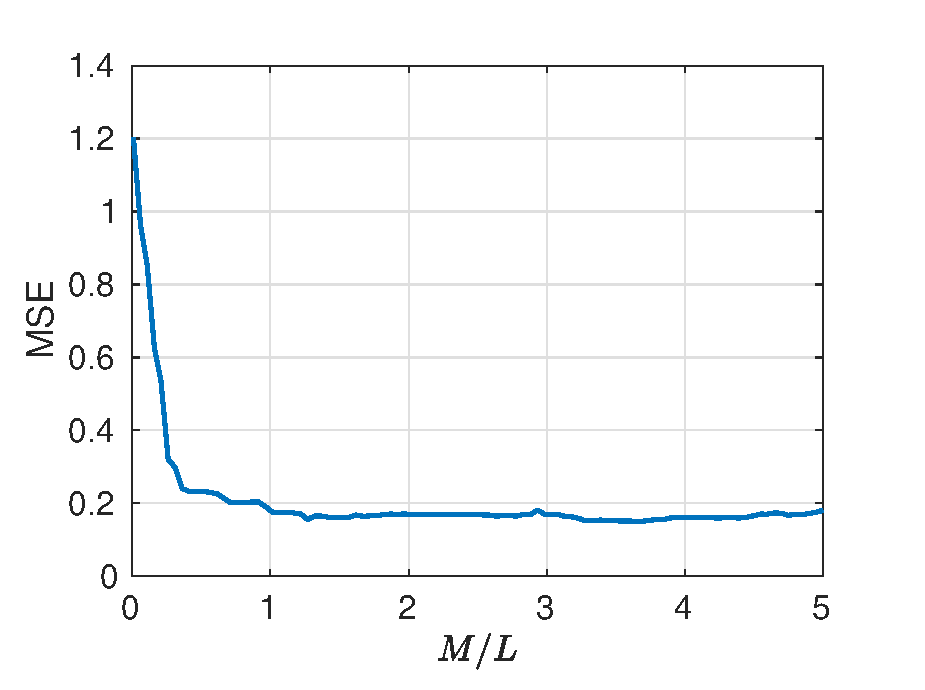
\includegraphics[width=.5\textwidth]{mseM.eps}
%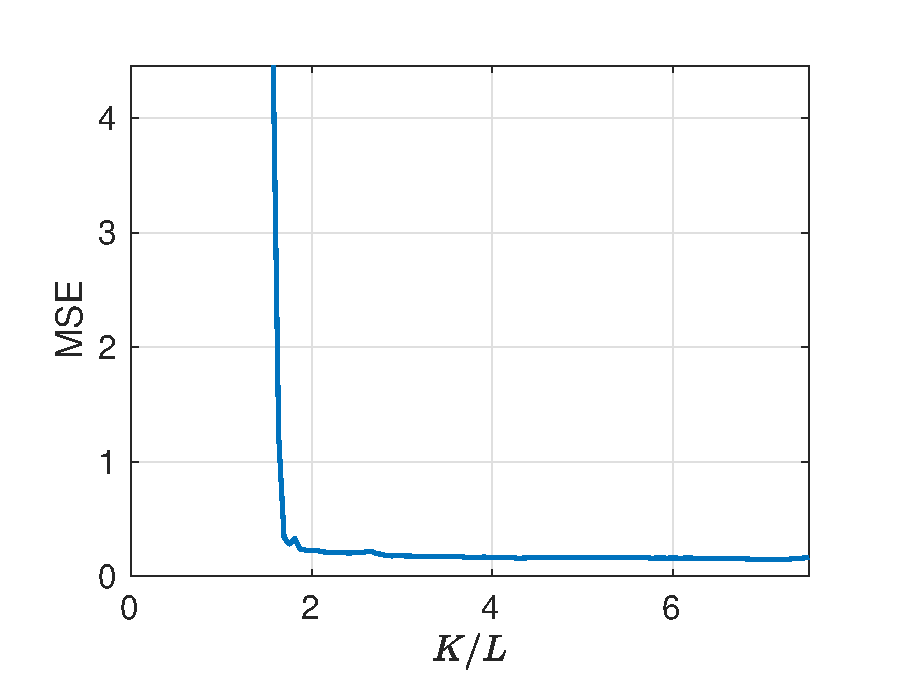
\includegraphics[width=.5\textwidth]{mseK.eps}
%\caption{Influence of the size parameters on the forecasting MSE. Left: MSE in function of the sub-signals length $M$. Right: MSE in function of the sub-signal dataset size $K$.}
%\label{fig:influence.M}
%\end{figure}

We divide the signal into 32-second long pieces, and apply Algorithm~\ref{alg:boundary} on each piece. We provide in Table~\ref{tab:otd.ppg} the OTD to the optimal time-frequency representation averaged over the signals. For all the considered time-frequency representations, the results clearly shows that our algorithm reduce the influence of the boundary effect. This highlights the ability of our approach to limit the distortion due the boundary effect and provide a more accurate representations.

On Fig.~\ref{fig:ppg.boundeffred}, we display the SST resulting from {\sf BoundEffRed} strategy, applied to the same portion of PPG than what is used to display Fig.~\ref{fig:ppg}. We clearly observe an improvement of the quality of the STT near boundaries. Indeed, the blurring visible on the zoom on the right boundary of the SST has almost vanished (see right of Fig.~\ref{fig:ppg.boundeffred}). The real-time tracking of the instantaneous frequencies contained the measured signal is therefore largely facilitated.    

\begin{table}
\centering
\caption{Performance of the Boundary effect reduction on TFR.}
\begin{tabular}{|c||c|c|c|}
  \hline
   \multirow{2}{*}{Extension method} & \multicolumn{3}{c|}{Time-Frequency Representation} \\
   \cline{2-4}
      & STFT & SST & RS\\
   \hhline{|=#=|=|=|}
   Without extension & $2.52\times 10^{-2}$ & $9.41\times 10^{-2}$ & $1.03\times 10^{-1}$ \\
   \hline
   {\sf SigExt} & $1.22\times 10^{-3}$ & $7.31\times 10^{-2}$ & $1.11\times 10^{-1}$ \\
   \hline
   EDMD & $9.83\times 10^{-4}$ & $5.59\times 10^{-2}$ & $9.80\times 10^{-2}$ \\
   \hline
   GPR & $1.14\times 10^{-3}$ & $7.02\times 10^{-2}$ & $1.07\times 10^{-1}$ \\
   \hline
\end{tabular}
\label{tab:otd.ppg}
\end{table}